\documentclass[pdf,mia,noFooter,slideColor,colorBG]{prosper}

\usepackage{amsmath}



\begin{document}

\title{Title}
\subtitle{Subtitles}
\author{Smurf}
\email{smurf@inra.fr}
\institution{INRA}

%\maketitle

\begin{slide}{}
\psline[linewidth=50pt,linecolor=white](-2,1.4)(10.3,1.4)
\rput[lb](2.5cm,0.4cm){\includegraphics[width=5cm]{Page1_top.eps}}
 \rput[lb](-0.3cm,-1.4cm){\includegraphics[width=10.5cm]{logoMIA19x2.eps}}
  \rput[lb](0.8cm,-4.8cm){Evaluation of the MIA Department -- October 2006}
 \rput[lb](-1.8cm,-5.2cm){\rotatebox[origin=c]{0}{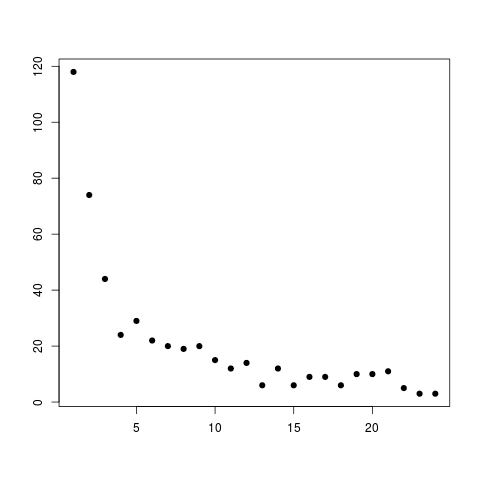
\includegraphics[width=2cm]{butterfly.eps}}}
\rput[lb](-2cm,-7.35cm){\includegraphics[width=13.7cm]{Page1_bottom.eps}}

  \rput[lb](1.9cm,-2.1cm){\Large\textbf{Title... (Helvetica)}}
\end{slide}


\begin{slide}{The quest for $\pi$}
\begin{itemize}
\item The following formula computes $8$ correct digits per iteration 
  (Ramanujan):
\end{itemize}
  \begin{small}
  \begin{equation*}
    \frac{1}{\pi}=\sum_{n=0}^\infty \frac{(\frac{1}{4})_n(\frac{2}{4})_n(\frac{3}{4})_n}{n!^3}\bigl(2\sqrt{2}(1103+26390n)\bigr)\frac{1}{(99^2)^{2n+1}}
  \end{equation*}
  \end{small}
\end{slide}

\end{document}
